%
% Chapter 4
%
\chapter{Implemented Infrastructure} \label{cap:implemented-infrastructure}

This chapter details the infrastructure implemented for the Remote Lab platform, covering the main components, technologies, deployment strategy, and integration between system modules.

\section{Overview}

The Remote Lab platform is designed as a modular, containerized system that enables secure and efficient remote access to laboratory equipment. The infrastructure follows a layered architecture, separating the user interface, backend logic, and hardware integration, and is built with scalability and maintainability in mind.

\begin{figure}[h]
    \begin{center}
        \resizebox{16cm}{!}{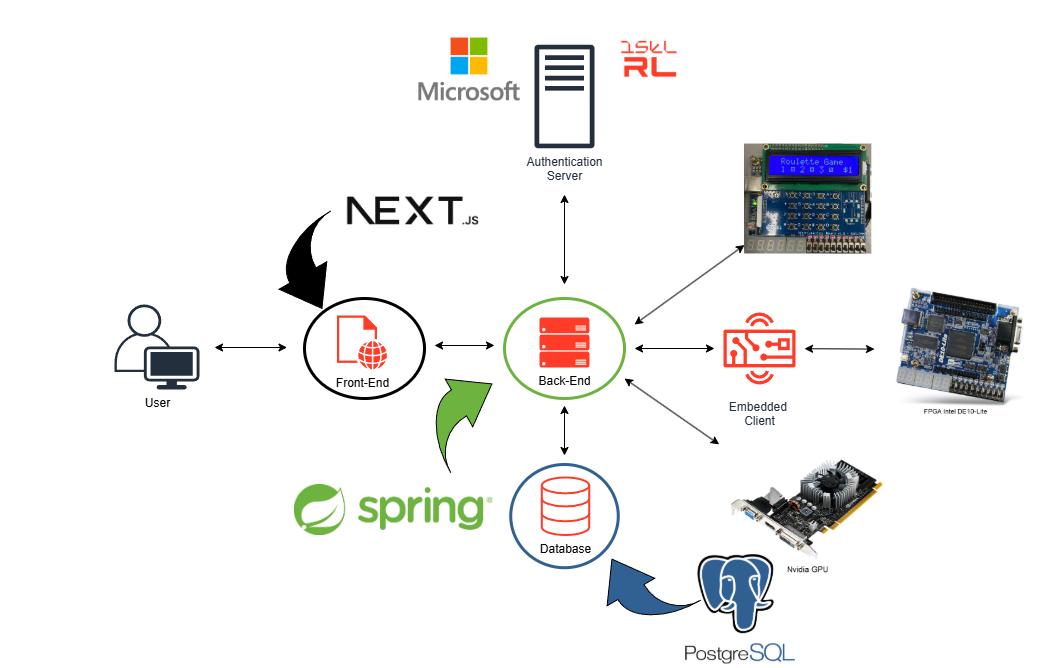
\includegraphics{../img/SystemArchitectureWithTechRL.png}}
    \end{center}
    \caption{System Architecture Overview}
    \label{fig:system-architecture}
\end{figure}

\section{Project Structure}
Project structure explaination.

\section{Implementation Details}
Project decisions.

\section{Database}
Database

\section{Web API}
Web API

\section{Web Application}
Web App

\section{Deployment}

\section{Technologies Used}

\begin{itemize}
    \item \textbf{Frontend:} Implemented with Next.js (React framework), providing a modern, responsive web interface for users to interact with laboratories, schedule sessions, and control hardware.
    \item \textbf{Backend:} Developed in Kotlin using Spring Boot, exposing RESTful APIs for user management, authentication, laboratory session control, and business logic enforcement.
    \item \textbf{Database:} PostgreSQL is used to persist user data, session information, access logs, and configuration settings.
    \item \textbf{ORM/Database Access:} JDBI is used for type-safe, modular database access in the backend.
    \item \textbf{Authentication:} Microsoft OAuth via NextAuth is used for user authentication, supporting multiple roles (student, professor, administrator).
    \item \textbf{Containerization:} Docker is used to containerize all major components (frontend, backend, database), ensuring consistent deployment across environments.
    \item \textbf{Orchestration:} Docker Compose manages multi-container deployment, networking, and environment configuration.
\end{itemize}

\section{System Components}

\begin{itemize}
    \item \textbf{Web Application (Frontend):} Provides dashboards, laboratory access, real-time hardware monitoring, and session management. Built with Next.js and deployed as a Docker container.
    \item \textbf{API Server (Backend):} Handles authentication, authorization, laboratory and user management, and hardware abstraction. Built with Kotlin and Spring Boot, also containerized.
    \item \textbf{Database:} PostgreSQL instance running in a Docker container, with persistent storage volumes.
    \item \textbf{Hardware Abstraction Layer:} Backend modules abstract hardware-specific details, exposing unified interfaces for laboratory equipment control.
\end{itemize}

\section{Deployment Architecture}

The system is deployed using Docker Compose, which defines and manages the following services:

\begin{itemize}
    \item \textbf{db:} PostgreSQL database container, with health checks and persistent volumes.
    \item \textbf{api:} Backend API container, built from the Kotlin/Spring Boot project, depending on the database service.
    \item \textbf{website:} Frontend container, built from the Next.js project, depending on the API service.
\end{itemize}

All services are connected via Docker networks to ensure secure and efficient communication. Environment variables and secrets are managed via \texttt{.env} files.

\section{Build and CI/CD}

\begin{itemize}
    \item \textbf{Gradle:} Used for building and managing backend dependencies.
    \item \textbf{NPM:} Used for frontend dependency management and builds.
    \item \textbf{Dockerfiles:} Multi-stage builds are used for both backend and frontend to optimize image size and security.
    \item \textbf{GitHub Actions:} (If applicable) Used for continuous integration and automated builds.
\end{itemize}

\section{Notable Implementation Details}

\begin{itemize}
    \item The backend uses JDBI for database access, configured with application-specific requirements.
    \item Environment variables are used to configure database connections and secrets, improving security and flexibility.
    \item The system supports role-based access control, with different permissions for students, professors, and administrators.
    \item The hardware abstraction layer allows for future extension to new types of laboratory equipment.
\end{itemize}

\section{Summary}

The implemented infrastructure leverages modern web technologies, containerization, and modular design to provide a robust, scalable, and maintainable platform for remote laboratory access.